\newSec[Signals]{Signalverarbeitung}{2}


\newSec[SignalsOffsetCalc]{Ermittlung der dauerhaften Nullpunkt-Abweichung}{3}
In \refImg{fig:SzeneOffset} wird eine Abweichung der Beschleunigungswerte vom Nullpunkt deutlich. Die eingesetzte Software wirkt dem in der \CodeClass{StateBuilder} entgegen, indem über eine definierte Anzahl an Eingangswerten der \CodeClass{IMUState} ein Mittelwert gebildet wird. Um an dieser Stelle aussagekräftigere Ergebnisse zu erhalten, wird zudem die Varianz über den zwischengespeicherten Datensatz gebildet. Der Mittelwert mit der geringste Varianz aus einer definierten Anzahl an Stichproben wird als Nullpunkt-Abweichung angenommen. Hierbei ist zu beachten, dass die Attribute der \CodeClass{IMUState} separat betrachtet werden.

\begin{figure}[ht!]
\vspace{0.25cm}
\begin{center}
\fbox{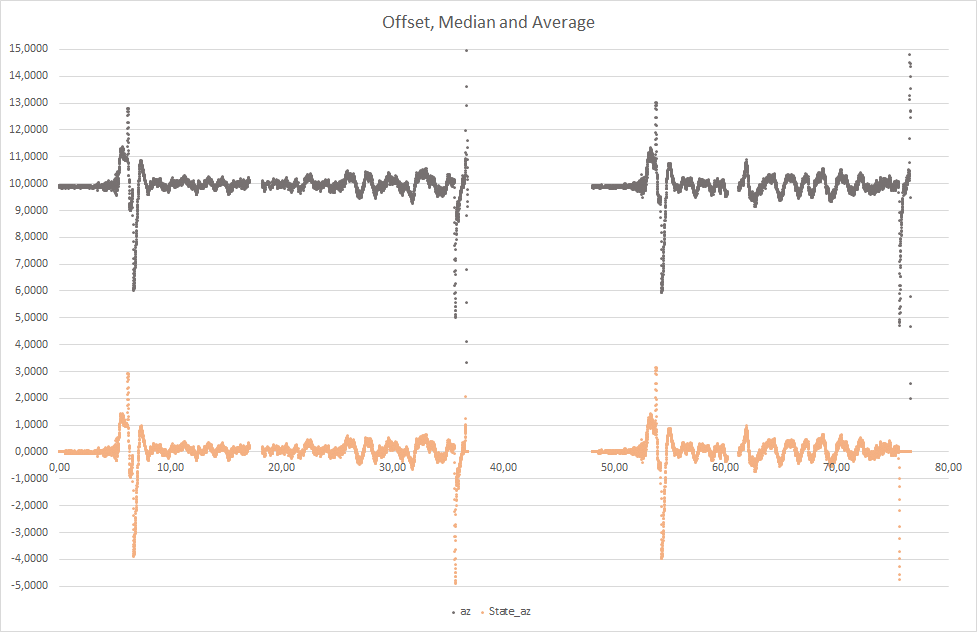
\includegraphics[width=12cm]{Pictures/TestFlight State_az Med1 Avg1 Off50 Calib1.png}}
\caption{Testflug Signalverarbeitung: Aufarbeitung $a_z$}
\label{fig:FlightStatusaz}
\end{center}

\vspace{0.25cm}
\refImgShort{fig:FlightStatusaz} zeigt die erfolgreiche Ermittlung der dauerhaften Nullpunkt-Abweichung für die Beschleunigungswerte entlang der z-Achse.\\
Es zeigt sich, dass die Nullpunkt-Abweichung aus den Eingangsdaten der \Quad-IMU berechnet und als Grundlage für eine weitere Aufarbeitung der Daten eingesetzt werden kann.
\end{figure}


\newSec[SignalsSmooth]{Glättung der Eingangsdaten}{3}
Als Parameter werden für die Berechnung der dauerhaften Nullpunkt-Abweichung (siehe \refCap{SignalsOffsetCalc}) jeweils ein Median-Fenster und ein Mittelwert-Fenster der Größe 1 angesetzt, somit findet keine Veränderung durch diese Filter statt. Es zeigte sich in den Auswertungen, dass ein Median-Fenster bis zur Größe von 15 Werten keinen signifikanten Einfluss auf die berechnete Pose besitzt. Jedoch wirkt sich eine Vergrößerung des Mittelwert-Fensters negativ auf die berechnete Pose aus. Die Abweichung von erwarteten Werten nimmt deutlich zu.


\newSec[SignalsOffsetCalib]{Kalibrierung der Posenberechnung}{3}
Aus Simulationen mit der in \refCap{Implementierung} beschrieben Software zeigte sich, dass eine einfach Abschätzung der Nullpunkt-Abweichung unach \refCap{SignalsOffsetCalc} nicht vollständig ausreicht. Der Einfluss bereits kleiner Nullpunkt-Abweichung wurde in \refCap{ControlPosAccelOffset} erläutert. Aus Erkenntnissen, aufgezeigt in \refImg{fig:SzeneOffset}, lässt sich nachfolgender mathimatische Zusammenhang ableiten:

\begin{equ}[!ht]
\begin{equation}
\Delta P_{Direction}=\frac{\Delta a_{Direction}}{2}*\Delta t^2
\end{equation}
\label{equ:OffsetCalib}
\caption{mathematische Grundlage der \textit{PoseBuildable}-Kalibrierung}
\end{equ}

Entsprechend dieser Formel berechnet die \CodeClass{PoseBuilder} eine nach der Aufarbeitung durch die \CodeClass{StateBuilder} verbleibende Nullpunkt-Abweichung der Beschleunigungswerte. Diese werden zur Berechung der Pose von den Eingangdaten subtrahiert.

In \refImg{fig:FlightPoseVel} kann gezeigt werden, dass sich eine zusätzliche Kalibrierung der Beschleungungsdaten positiv auf die Berechnung der Pose\footnote{In der genannten Abbildung werden die berechneten Geschwindigkeiten aufgetragen.} auswirken kann. Die durch die \CodeClass{PoseBuildable} berechnete Geschwindigkeit entlang der z-Achse entspricht für den zweiten Flug etwa der aus dem gemessenen Höhenverlauf abgeleiteten Geschwindigkeit.

\begin{figure}[ht!]
\vspace{0.25cm}
\begin{center}
\fbox{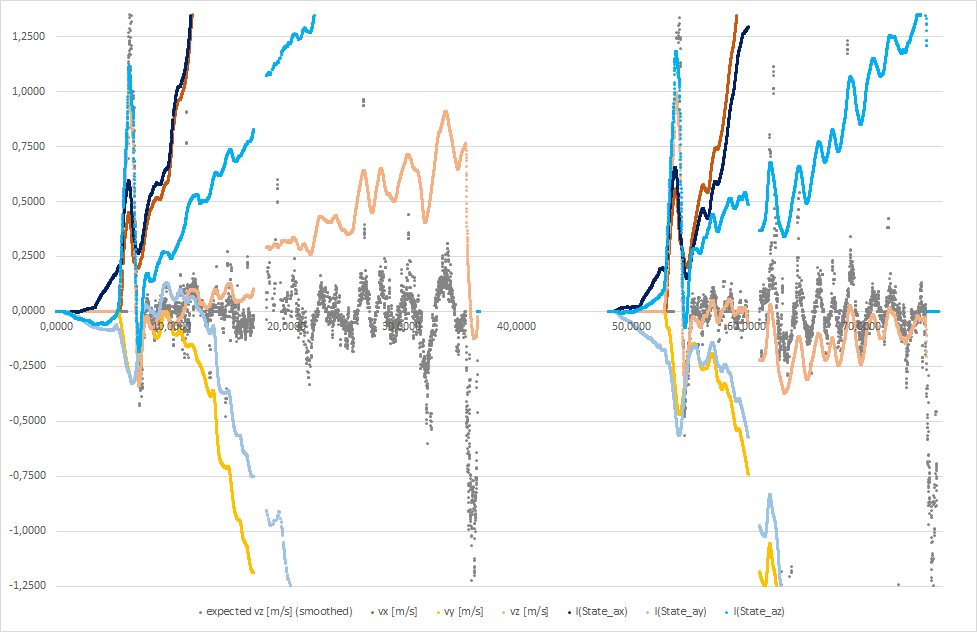
\includegraphics[width=15cm]{Pictures/TestFlight Velocity Med1 Avg1 Off50 Calib1.png}}
\caption{Testflug Signalverarbeitung: Kalibrierung}
\label{fig:FlightPoseVel}
\end{center}

\vspace{0.25cm}
An der aufgetragenen Geschwindigkeit \textit{vz} lässt sich deutlich erkennen, welchen Einfluss die Kalibrierung der \CodeClass{PoseBuildable} hat. Die berechnete Geschwindigkeit (beige) weicht nur mäßig von der erwarteten Geschwindigkeit (grau) ab.\\
\note{Da die \textit{IMU}-Nachrichten in einer Folgen mit kurzen Zeitschritten eintreffen, wurde die erwartete Geschwindigkeit als gleitender Mittelwert über 10 Werte geglättet.}
\end{figure}



















